\documentclass[letter, 10pt]{article}
\usepackage[utf8]{inputenc}
\usepackage[spanish]{babel}
\usepackage{amsfonts}
\usepackage{amsmath}
% \usepackage[dvips]{graphicx}
\usepackage{graphicx}
\usepackage{url}
\usepackage{hyperref}
\usepackage[top=3cm,bottom=3cm,left=3.5cm,right=3.5cm,footskip=1.5cm,headheight=1.5cm,headsep=.5cm,textheight=3cm]{geometry}
\usepackage{multirow}
\usepackage{algorithm}
\usepackage[noend]{algpseudocode}
\usepackage{listings}

\lstdefinestyle{myBash}{
basicstyle=\small,
language=bash,
captionpos=b, 
label=lst:4, 
frame=LRTB,
breaklines=true,
showtabs=true, 
% escapechar=@
}

\usepackage[table,xcdraw]{xcolor}

\usepackage{todonotes}

\renewcommand{\algorithmicrequire}{\textbf{Input:}}
\renewcommand{\algorithmicensure}{\textbf{Output:}}


\begin{document}
\title{Inteligencia Artificial \\ \begin{Large}Estado del Arte: \textbf{Weapon target assignment problem}\end{Large}}
\author{Pedro Donoso Aguilera}
\date{\today}
\maketitle


%--------------------No borrar esta secci\'on--------------------------------%
\section*{Evaluaci\'on}

\begin{tabular}{ll}
Resumen (5\%): & \underline{\hspace{2cm}} \\
Introducci\'on (5\%):  & \underline{\hspace{2cm}} \\
Definici\'on del Problema (10\%):  & \underline{\hspace{2cm}} \\
Estado del Arte (35\%):  & \underline{\hspace{2cm}} \\
Modelo Matem\'atico (20\%): &  \underline{\hspace{2cm}}\\
Conclusiones (20\%): &  \underline{\hspace{2cm}}\\
Bibliograf\'ia (5\%): & \underline{\hspace{2cm}}\\
 &  \\
\textbf{Nota Final (100\%)}:   & \underline{\hspace{2cm}}
\end{tabular}
%---------------------------------------------------------------------------%
\vspace{2cm}

\begin{abstract}
En este informe se expondrá un problema relacionado a la estrategia militar, más específicamente la asignación de armas a objetivos de guerra. Este problema conocido como \textit{Weapon Target Assignament Problem} (WTA) tiene diversas formas de obtener una solución, una técnica incompleta bastante eficiente \cite{andersen-2022} es \textit{Branch and Bound} utilizando relajación y también se han encontrado técnicas incompletas que encuentren óptimos locales que se trabajarán más adelante.
Lo que se busca es que el lector comprenda la formulación de la problemática y la implementación de una de las técnicas incompletas utilizando heurísticas para mejorar la búsqueda del óptimo local
 con la finalidad de entender que no existe un solo método para solventar un problema, sino que es posible combinar o crear heurísticas para encontrar óptimos locales que nos entreguen soluciones de calidad.
\end{abstract}

\section{Introducci\'on}
% Una explicaci\'on breve del contenido del informe, es decir, detalla: Prop\'osito, Estructura del Documento, Descripci\'on (muy breve) del Problema y Motivaci\'on.

\subsection{Propósito}
Este informe fue desarrollado con el propósito de que lector conozca que existen diferentes forma de abordar un problema de optimización combinatoria, específicamente el problema de asignación de armas a objetivos de guerra, para que así pueda aplicar este conocimiento en problemas similares.

\subsection{Descripción del problema}

% En esta sección no hay citas/referencias a otros artículos que respalden la información presentada.

% No se mencionan problemas relacionados, como por ejemplo el assignment problem, que es el problema general de asignación en la literatura.

En este informe se dispondrá al lector un problema relacionado con las estrategias de guerra, específicamente el problema de Asignación de objetivos de armas, este problema conocido como \textit{Weapon Target Assignment} (WTA) consiste en la asignación de armas amigas a los objetivos hostiles con el fin de proteger los activos amigos o destruir los objetivos hostiles, es considerado un problema NP-completo, por consiguiente tiene variaciones en su formulación y diversas formas de obtener una solución.
Este documento busca expresarle al lector la esencia del problema para luego estudiar las diversas formas de encontrar soluciones incompletas, heurísticas a utilizar y compararlas, comprendiendo así que no sólo existe una forma para encontrar soluciones.

\subsection{Estructura del documento}
% No se presenta la estructura del documento.
Primero se presentará la Definición del problema, donde se explicará el caso general del problema de una manera verbal para que sea entendido fácilmente y se tenga una idea general de este informe. En segundo lugar se tendrá el Estado del Arte, donde se mostrarán los estudios realizados con antelación, con la finalidad de proveer al lector información relevante que le sirva para ver las diferentes formas de abordar el problema de optimización combinatoria.
En tercer lugar estarán los Modelos Matemáticos tanto para el caso general del WTA como para un caso específico de este, es necesario tener presenta las variables, restricciones y funciones objetivo para poder utilizar los algoritmos que se presentarán en el documento. Por último se tendrán las Conclusiones, que comparará los métodos planteados en el informe y se dará un pequeño resumen del más prometedor. 

\subsection{Motivación}
La motivación para crear este informe es aprender como un problema puede ser resuelto de diferentes formas, con el fin de posteriormente intentar crear una solución al WTA recurriendo al conocimiento extraído de este informe, ya sea utilizando una de esas técnicas o combinándolas.


\section{Definición del Problema}
% Explicación del problema
% En qué consiste
% Cuales son su variables
% Probablidades
% Restricciones 
% Funcion objetivo
% Problemas relacionados.
% variantes más conocidas

El problema nacido a mediados del siglo XX, introducido por la necesidad de ventaja militar en la época, llamado Problema de Asignación  de Objetivos de Armas, más conocido como \textit{Weapon Target Assignment Problem} (WTA) es una clase de problemas de optimización combinatoria presentes en los campos de optimización e investigación de operaciones.
El problema anterior nace como una variación del problema de asignación, conocido como \textit{Assignment Problem} (AP), problema fundamental de los denominados problemas de optimización combinatoria.

% ¿Qué trabajos son parte de esta categoría? Para justificar estas aseveraciones es necesario incluir citas a trabajos específicos.
%  \cite[pág 21]{Introduccion}
%  \cite[pág 21]{Background}
%  \cite[pág 21]{WithTechniques}

Es bastante común encontrar en la literatura sobre el WTA que se centra en la perspectiva defensiva \cite{ahuja-2007}    \cite{Introduccion} \cite{WithTechniques}, encontrar la asignación óptima de armas a las amenazas de una manera que minimice el daño esperado, pero es inevitable que algunos consideren la perspectiva ofensiva \cite{Background}, encontrar una asignación óptima de un conjunto de armas de varios tipos a un conjunto de objetivos para maximizar el daño total esperado infligido al oponente.
Para cuestiones de este acercamiento al problema consideraremos su perspectiva defensiva.

El problema básico consiste en considerar una cantidad de tipos de armas y objetivos, a cada objetivo se le asigna un valor destructivo, disponemos también de la probabilidad de destrucción de los objetivos para la asignación de armas y objetivos, por otra parte, restringiendo el espacio de búsqueda debemos considerar que la cantidad de armas disponibles y la cantidad mínima de armas requeridas en cada objetivo condicionan la cantidad de armas asignadas a cada objetivo, esto para asegurarnos de que  el número total de armas utilizadas no exceda la cantidad de armas disponibles. 
También debemos tener en cuenta que cada objetivo deba tener al menos 1 arma asignada y que no podemos asignar más de 1 arma por objetivo.


% Esta es una de las restricciones que podemos encontrar. Existen más restricciones que podemos hallar según la formulación del problema, como que cada objetivo deba tener al menos 1 arma asignada, o que no podemos asignar más de 1 arma por objetivo, entre otras.

Nuestro objetivo es minimizar el valor esperado de supervivencia, es decir, minimizar el valor de daño para cada objetivo teniendo en cuenta la probabilidad de que cierta arma no destruya cierto objetivo y su valor destructivo.

Antes de explicar las diferentes variaciones de este problema debemos definir lo que es un escenario o etapa, esto es una iteración donde se realiza una evaluación de los daños, y en base a esta evaluación se reasignan las armas disponibles a los objetivos supervivientes de forma iterativa.

En la literatura podemos encontrar diferentes variaciones de este problema, por ejemplo, la multi-objetivo, donde se puede asignar más de un arma a cada objetivo y no se requiere que todos los objetivos tengan armas asignadas. Además, tenemos las variaciones más comunes, el problema WTA estático y dinámico.
En el caso estático, las armas se asignan a los objetivos una vez, por el contrario el caso dinámico implica agregar el tiempo como una dimensión adicional, los escenarios posteriores se verán relacionados directamente por el escenario anterior, así irá modificándose a medida que avanza el tiempo.

Para este trabajo se considerará la variación más simple, el problema WTA estático y no se utilizará ningún proceso de defensa iterativo, es decir, se pasará un escenario inicial y se trabajará siempre con ese mismo, no cambiará con el transcurso de la búsqueda.
% Esto corresponde a la variante dinámica del problema. La versión estática asigna armas a objetivos conocidos en un solo paso, sin iteraciones posteriores.

%que existe cierta capacidad de cada arma para atacar múltiples objetivos al mismo tiempo, 
% queremos encontrar la cantidad de armas de cada tipo asignadas a cierto objetivo, teniendo en cuenta la probabilidad de que cierta arma destruya cierto objetivo.
% Función objetivo es minimizar el valor esperado de supervivencia, es decir, minimizar el valor de daño para cada objetivo

\section{Estado del Arte}

% qué métodos se han usado para resolverlo?
% cuáles son los mejores algoritmos que se han creado hasta la fecha?
% qué representaciones han tenido los mejores resultados?
% cuál es la tendencia actual para resolver el problema?
% tipos de movimientos
% heurísticas
% métodos completos
% tendencias
% incluye gráficos comparativos o explicativos

% No hay justificación para esta decisión, la sección del estado del arte es la más importante en esta entrega y la que amerita mayor discusión y opinión propia del alumno.

% No se discute acerca de las representaciones usadas en los experimentos.

% No se expresan conclusiones respecto al por qué de los resultados mostrados. Se debe explicar por qué ciertas técnicas funcionan mejor que otras y bajo qué formulaciones del problema.

% No se discute acerca de tendencias de nuevas investigaciones

% Solo se toma en cuenta un resultado de un experimento y no se analizan las técnicas por separado.


En esta sección del trabajo no se discutirán los detalles de los algoritmos estudiados, porque no es parte esencial de este trabajo, solamente se dispondrá información recopilada sobre las diferentes técnicas utilizadas en la literatura para resolver de la forma más óptima este problema combinacional.
Los algoritmos estudiados serán Tabu Search, Simulated Annealing, Genetic Algorithm y Variable Neighborhood Search.

% Figuras mal organizadas
En al figura \ref{fig_comparison} se muestra una comparación realizada en un estudio del problema de los algoritmos antes mencionados, dispuestos como TS, SA, GA y VNS, este gráfico nos muestra el tiempo en unidades de CPU de estos algoritmos a medida que aumentan las iteraciones o escenarios, con un máximo de 19 escenarios.

Se puede notar que los valores de tiempo de CPU se aproximan hasta el escenario 10, después, hay pendientes pronunciadas para GA, TS y especialmente para VNS.
EL tiempo de solución de SA tiene una pendiente muy baja y se puede ver fácilmente que SA supera a estos algoritmos cuando la dimensión del problema es mayor.


\begin{figure}[!ht]
    \centering
    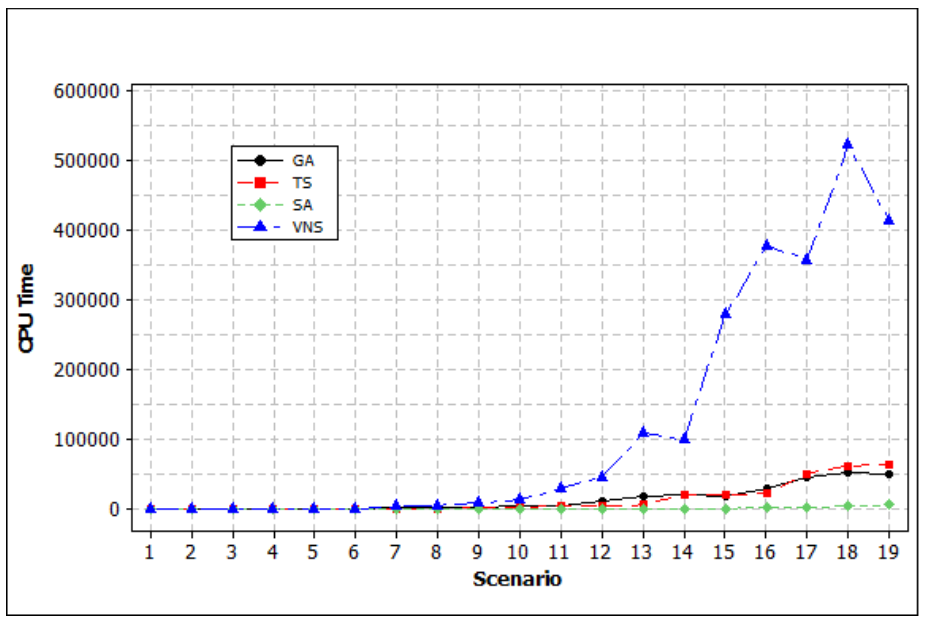
\includegraphics[width=0.8\textwidth]{images/cpu_time_comparasion_of_algorithms.png}
    \caption{CPU Time Comparison of Algorithms \cite[pág 47]{WithTechniques}}
    \label{fig_comparison}
\end{figure}

% \subsection{Genetic Algorithm}
% \subsection{Tabu Search}
% \subsection{Simulated Annealing}
% \subsection{Variable Neighborhood}


\section{Modelo Matem\'atico}
% Uno o m\'as modelos matem\'aticos para el problema, idealmente indicando el espacio de b\'usqueda para cada uno. Cada modelo debe estar correctamente referenciado, adem\'as no debe ser una imagen extraida. Tambi\'en deben explicarse en detalle cada una de las partes, mostrando claramente la funci\'on a maximizar/minimizar, variables y restricciones. Tanto las f\'ormulas como las explicaciones deben ser consistentes.

% ¿De dónde se obtuvo el modelo?

Para expresar matemáticamente esta variación estática del problema WTA, de ahora en adelante denotada como SWTA, extraída del paper guía llamado  \href{https://web.karabuk.edu.tr/emrullahsonuc/wta/A_Parallel_Simulated_Annealing_Algorithm_for_Weapon-Target_Assignment_Problem.pdf}{A Parallel Simulated Annealing Algorithm for Weapon-Target Assignment Problem}
  debemos definir primero que $i = 1, \dots , n$ corresponde a cada objetivo con $n$ la cantidad total de objetivos y $j = 1, \dots , m$ para cada objetivo con $m$ la cantidad total de tipos de armas.


\subsubsection{Parámetros}
Definiremos las siguientes variables.

\begin{align*}
    m :& \text{ número de objetivos a destruir.} \\
    n :& \text{ número de tipos de armas. Con un arma por cada tipo.} \\
    p_{ij}:& \text{ la probabilidad de que el arma} \; j \; \text{destruya el objetivo} \; i. \\
    % q_{ij}:& \text{la probabilidad de que el arma i no destruya el objetivo j} \\
    V_j :& \text{ el valor de destructivo del objetivo} \; j \\
    % K :& \text{el n\'umero de activos protegidos} \\
    % a_k :& \text{el valor del activo k} \\
    % n :& \text{ el número de objetivos} \\
    % m :& \text{ el número de tipos de armas} \\
    % \mathcal{W}_i :& \text{ el número de armas del tipo i} \\
    % c_{ij} :& \text{un par\'ametro de costo para asignar un arma del tipo i al objetivo j} \\
    % \mathcal{F} :& \text{el conjunto de asignaciones factibles} \\
    % \gamma_{jk} :& \text{la probabilidad de que el objetivo j destruya el activo k} \\
    % \mathcal{S}_j :& \text{el n\'umero m\'aximo de armas que pueden ser asignadas al objetivo j} \\
\end{align*}

\subsubsection{Variable}
La variable \ref{ec:variable_x} definida nos ayudará a representar nuestro escenario, para cuestiones matemáticas se representará como una variable binaria para mostrarnos a qué objetivo se le asigna el arma $i$.
Para cuestiones de representación en el algoritmo, será un arreglo que contenga el identificador del arma del tipo $j$ asignada al objetivo $i$, y cada casilla corresponderá a un objetivo distinto, esto nos permitirá tratar con la restricción mediante la representación. 

\begin{align}
    \mathcal{X}_{ij} :&  
    \left\lbrace 
    \begin{array}{l} 
    \text{Si el arma} \; j \; \text{es asignado a el objetivo} \; i \\ 
    0 \; \text{otro caso} 
    \end{array}
    \right.
    \label{ec:variable_x}
\end{align}

\subsubsection{Formulación SWTA}
Un defensor tiene $w_i = 1, ... , m$ tipos de armas con las que defenderse contra $j=1, ... , n$ objetivos.
Cada arma del tipo i tiene una probabilidad $p_{ij}$ de matar al objetivo $j$ y cada objetivo $j$ tienen un valor destructivo $V_j$.
Con las variables de decisi\'on $\mathcal{X}_{ij}$ indicando el n\'umero de armas de tipo $i$ para asignar al objetivo $j$, se formula el \textit{SWTA} de la siguiente manera. \cite[pág 2]{Background}

% No hay explicación de las restricciones ni de la función objetivo

\subsection{Función Objetivo}

Los pesos definidos los interpretamos según el autor del paper antes mencionado, como el valor destructivo, entonces buscaremos minimizar la suma ponderada de los pesos $\mathcal{V_i}$, es decir, minimizar los daños que recibiría el recurso que deseamos proteger.


\begin{align*}
    \textrm{min} & \sum^{n}_{j=1} \mathcal{V}_j \prod^{m}_{i=1}{(1 - p_{ij})^{\mathcal{X}_{ij}} }
\end{align*}

\subsection{Restricciones}

En la ecuación \ref{res:1} está representada la restricción relacionada con que cada objetivo debe tener asignada un arma y un arma debe estar relacionada con un objetivo. 

\begin{align}
    \label{res:1}
    \textrm{s.t.} & \, \sum^{n}_{j=1}{\mathcal{X}_{ij} } = 1 \,, \quad \textrm{for} \: i = 1, \dots, m \\
    \nonumber
    & \mathcal{X}_{ij} \in \mathds{Z}_{+} \,, \quad \textrm{for} \: i=1, \dots, m, \: j=1, \dots, n 
\end{align}

Más adelante nos daremos cuenta que esta restricción está tratada implícitamente por la representación.

\section{Representación}

Como entrada al algoritmo se tiene un archivo de texto que contiene en su primera linea la cantidad de objetivos y armas, que se le denominará dimensión de la instancia, para este caso de estudio será la misma cantidad de armas que de objetivos, en sus lineas siguientes especifica los valores de destrucción de cada objetivo y en las restantes, las probabilidades de que el arma de tipo $i$ destruya al objetivo $j$.

Como estructura de datos para representar la solución, se dispondrá de un arreglo del mismo largo que la cantidad de armas y objetivos, en cada índice se representará los objetivos y los valores de cada casilla representará el arma que se le asignó a cada objetivo, la justificación de ello tiene relación con la sección anterior.

Como se mencionó en la sección anterior, la restricción \ref{res:1} que acota la cantidad de armas asignadas a una por cada objetivo y viceversa, está tratada implícitamente en esta representación vectorial.

En el modelo matemático se representa $X_{ij}$ como una matriz bidimensional que indica la cantidad de cada arma relacionada con cada objetivo.

    \begin{table}[h!]
    \centering
    \begin{tabular}{ll|lll|}
    \cline{3-5}
     &  & \multicolumn{3}{l|}{Armas} \\ \cline{3-5} 
     &  & \multicolumn{1}{l|}{\textbf{0}} & \multicolumn{1}{l|}{\textbf{1}} & \textbf{2} \\ \hline
    \multicolumn{1}{|l|}{\multirow{3}{*}{Objetivos}} & \textbf{0} & 2 & 0 & 1 \\ \cline{2-2}
    \multicolumn{1}{|l|}{} & \textbf{1} & 1 & 3 & 0 \\ \cline{2-2}
    \multicolumn{1}{|l|}{} & \textbf{2} & 8 & 3 & 1 \\ \hline
    \end{tabular}
    \caption{Representación matricial de la solución.}
    \label{fig:rep_sol_matrix}
    \end{table}
    
Como se puede ver en la representación anterior \ref{fig:rep_sol_matrix}, los índices de las columnas, marcadas en negrita, representa cada tipo de arma con índices 0,1 y 2, y en las filas se representan los objetivos con índices 0,1 y 2, entonces podemos decir que al objetivo 0, se le asignan 2 armas del tipo 0, 0 armas del tipo 1 y 1 arma del tipo 2.

Esto ayuda a estandarizar una representación para los problemas del tipo WTA que permite tener más de un arma asignada a un objetivo, pero esto solo se representa así en este documento para la comprensión del lector, cuando se acota el dominio de los valores que se le asignan en cada casilla de la matriz  $X_{ij}$ al dominio de este caso particular de problema SWTA con un arma asignada para cada objetivo \ref{fig:rep_sol_matrix_bin}, entonces se puede generar una matriz diagonal que se aproxime más a lo que se necesita.


\begin{table}[h!]
    \centering
    \begin{tabular}{ll|lll|}
    \cline{3-5}
     &  & \multicolumn{3}{l|}{Armas} \\ \cline{3-5} 
     &  & \multicolumn{1}{l|}{\textbf{0}} & \multicolumn{1}{l|}{\textbf{1}} & \textbf{2} \\ \hline
    \multicolumn{1}{|l|}{\multirow{3}{*}{Objetivos}} & \textbf{0} & 1 & 0 & 0 \\ \cline{2-2}
    \multicolumn{1}{|l|}{} & \textbf{1} & 0 & 1 & 0 \\ \cline{2-2}
    \multicolumn{1}{|l|}{} & \textbf{2} & 0 & 0 & 1 \\ \hline
    \end{tabular}
    \caption{Representación matricial de la solución.}
    \label{fig:rep_sol_matrix_bin}
\end{table}

Con esto se puede evidenciar que no es necesario tener una matriz que representa una posible solución porque las casillas que representan los ceros están demás, consumen memoria y puede llegar a ser difícil de manejar, es por lo anterior que se modificó la representación de la posible solución a una representación vectorial.

\begin{table}[h!]
\centering
\begin{tabular}{lllll}
\textbf{0}              & \textbf{1}             & \textbf{2}             &           &           \\ \cline{1-3}
\multicolumn{1}{|l|}{2} & \multicolumn{1}{l|}{0} & \multicolumn{1}{l|}{1} & \textbf{} & \textbf{} \\ \cline{1-3}      
\end{tabular}

\caption{Representación vectorial de la solución.}
\label{fig:rep_sol_vector}
\end{table}

Entonces la nueva representación consiste en mostrar en cada casilla el tipo de arma que se le asigna a cada objetivo y los índices de dicho vector representan a los objetivos, de esta manera se utiliza mucho menos espacio en memoria y se puede manejar implícitamente la restricción \ref{res:1}, haciendo un movimiento de intercambio de posiciones (switch) por ejemplo.

\section{Descripción del algoritmo}

El algoritmo que se analizará es una implementación del algoritmo \textit{Simulated Annealing} en combinación con la heurística \textit{Best Improvement} o \textit{Mejor mejora}, esto se implementará como una especie de \textit{Hill Climbing}, dado que se generará un vecindario y de dicho vecindario se escogerá el mejor.

Luego de que se escoja el mejor se aplicará la lógica de \textit{SA}, entonces allí se decidirá con la temperatura y probabilidades si se acepta o no la solución.

Se seguirá de esta forma hasta que se logre la cantidad máxima de iteraciones o hasta que se llegue a una temperatura mínima.

Se debe tener en cuenta que $delta$ es el delta de la mejor solución escogida, $new\_solution$ es la solución a la que corresponder ese mejor $delta$ escogido y $k$ es coeficiente de decaimiento de la temperatura.

\begin{algorithm}[H]
\caption{\textit{Simulated Annealing} con \textit{Best Improvement}}
\label{alg:Framwork}  
  \begin{algorithmic}
    \Require WTA5.txt
    \Ensure Mejor solución
    \State -----------------------------------------------------
    \State Definir variables extraídas de parsear el archivo de texto, dimensión, probabilidades de destrucción y pesos.
    \State Definir temperatura inicial, temperatura mínima, su decaimiento y el máximo de iteraciones.
    \State Generar solución inicial
    \State Instanciar mejor solución y solución actual.
    \While {($numero\_iteraciones < maximo\_iteraciones$) and ($T\_current > T\_min$)}
    % \State Otorgar a cada solución una puntuación
    \State Generar movimientos de los índices de los vecinos
    \State Calcular los deltas de la solución actual y las soluciones con el movimiento.
    \State Escoger la solución que tenga mejor delta.
    \If{acceptance\_function( $delta$, $T\_current$)}
    \State accept\_solution( $problem$ , $new\_solution$ )
    \Else
    \State reject\_solution()
    \EndIf
    \State change\_temperature($T\_current$, $k$)
    \State $numero\_iteraciones + 1$
    \EndWhile
    \State Imprimir mejor solución y su calidad
  \end{algorithmic}
\end{algorithm}

Comenzamos definiendo nuestros parámetros iniciales y constantes a utilizar en el algoritmo, el vector de probabilidades de destrucción y el vector que representa los valores destructivos delos objetivos extraídos de la instancia definida al ejecutar el algoritmo, en esta primera parte también definimos las temperaturas inicial y final, el coeficiente de decaimiento de la temperatura y el máximo de iteraciones.

Iniciando con el algoritmo, generamos una solución inicial definida como la correspondencia secuencial de cada arma a su respectivo objetivo, es decir, el arma 2 asignada al objetivo 2, y así sucesivamente, en un vector en dos dimensiones correspondería a la matriz diagonal.
Luego le sigue el bucle que ayudará a realizar la búsqueda, con dos sentencias de control de flujo, una que controla la cantidad de iteraciones y otra que controla que se esté trabajando dentro de los rangos acordados de temperatura.

En la búsqueda se genera el vecindario aplicándole un movimiento diferente a la solución actual, se calculan los deltas de cada vecino, se escoge la solución con el mejor delta y con este delta se realiza el proceso de aceptación de la solución escogida. Si se acepta la solución, es guardada como la mejor hasta el momento y si se rechaza, se sigue con la misma mejor solución con la que se inició la iteración de búsqueda, para finalizar la iteración se cambia la temperatura multiplicando la temperatura actual por el coeficiente de decaimiento.

Con respecto a la búsqueda el movimiento que se le realiza a cada vecino se realiza en base a un objetivo pivot escogido aleatoriamente, esto ayuda a realizar los movimientos swap a todos los vecinos, por ejemplo, en una instancia de 5 dimensiones, se escoge un pivot 2, y se cambia cada objetivo por el del pivot, generando 4 vecinos \ref{fig:gen_vecindario}.



\begin{table}[h!]
\centering
\begin{tabular}{llllll}
\hline
\multicolumn{1}{|l|}{Solución Inicial} & \multicolumn{1}{l|}{0} & \multicolumn{1}{l|}{1} & \multicolumn{1}{l|}{\cellcolor[HTML]{9AFF99}2} & \multicolumn{1}{l|}{3} & \multicolumn{1}{l|}{4} \\ \hline
 &  &  &  &  &  \\ \hline
\multicolumn{1}{|l|}{Vecino 0} & \multicolumn{1}{l|}{\cellcolor[HTML]{9AFF99}2} & \multicolumn{1}{l|}{1} & \multicolumn{1}{l|}{\cellcolor[HTML]{FFCCC9}0} & \multicolumn{1}{l|}{3} & \multicolumn{1}{l|}{4} \\ \hline
\multicolumn{1}{|l|}{Vecino 1} & \multicolumn{1}{l|}{0} & \multicolumn{1}{l|}{\cellcolor[HTML]{9AFF99}2} & \multicolumn{1}{l|}{\cellcolor[HTML]{FFCCC9}1} & \multicolumn{1}{l|}{3} & \multicolumn{1}{l|}{4} \\ \hline
\multicolumn{1}{|l|}{Vecino 2} & \multicolumn{1}{l|}{0} & \multicolumn{1}{l|}{1} & \multicolumn{1}{l|}{\cellcolor[HTML]{FFCCC9}3} & \multicolumn{1}{l|}{\cellcolor[HTML]{9AFF99}2} & \multicolumn{1}{l|}{4} \\ \hline
\multicolumn{1}{|l|}{Vecino 3} & \multicolumn{1}{l|}{0} & \multicolumn{1}{l|}{1} & \multicolumn{1}{l|}{\cellcolor[HTML]{FFCCC9}4} & \multicolumn{1}{l|}{3} & \multicolumn{1}{l|}{\cellcolor[HTML]{9AFF99}2} \\ \hline
\end{tabular}
\caption{Vecindario generado en base a la solución inicial de ejemplo}
\label{fig:gen_vecindario}
\end{table}




\section{Experimentos}

Antes de comenzar cualquier proceso de experimentación se deben explicitar los óptimos locales propuestos por la literatura de referencia \cite{sonuc-2017}.

\begin{table}[!ht]
\centering
\begin{tabular}{|l|l|llll}
\cline{1-2}
\textbf{Instancia} & \textbf{Mejor SA} &  &  &  &  \\ \cline{1-2}
5 & 48.3640 &  &  &  &  \\ \cline{1-2}
10 & 96.3123 &  &  &  &  \\ \cline{1-2}
20 & 142.1070 &  &  &  &  \\ \cline{1-2}
30 & 248.0285 &  &  &  &  \\ \cline{1-2}
40 & 305.5016 &  &  &  &  \\ \cline{1-2}
50 & 353.0767 &  &  &  &  \\ \cline{1-2}
60 & 415.0528 &  &  &  &  \\ \cline{1-2}
70 & 498.1049 &  &  &  &  \\ \cline{1-2}
80 & 534.4408 &  &  &  &  \\ \cline{1-2}
90 & 594.0639 &  &  &  &  \\ \cline{1-2}
100 & 699.8357 &  &  &  &  \\ \cline{1-2}
200 & 1306.9126 &  &  &  &  \\ \cline{1-2}
\end{tabular}
\caption{Mejores óptimos locales de literatura de referencia.}
\label{tab:optimos_ref}
\end{table}

Durante todos los experimentos realizados se utiliza esta información para comparar implementaciones de algoritmos.

\subsection{Metodología}

Para poner a prueba este algoritmo y encontrar el mejor óptimo local se realizaron diferentes experimentos de sintonización de parámetros, acordando al menos 5 iteraciones de ejecución del algoritmo como una cantidad razonable para evidenciar el alcance de las pruebas con temperatura y al menos 10 iteraciones para las pruebas con movimientos, lo anterior para lograr realizar los experimentos en menos de una hora, tiempos totales que se documentaron en los archivos excel adjuntos en la carpeta \textit{stadistics} los parámetros a sintonizar en estos experimentos son los siguientes:

\begin{itemize}
    \item Movimiento.
    \item Temperatura y coeficiente de decaimiento.
\end{itemize}

Cabe destacar que para realizar de forma más óptima este proceso de sintonización se modificó el algoritmo para que se pasasen los parámetros por argumentos. Además para realizar el cambio de parámetros se compiló el código y se llamó a la función \textit{run} del Makefile que nos permite entregarle los parámetros con nombre al algoritmo, esto simplemente se hace con fines demostrativos, simplemente se podría pasar los parámetros directamente al ejecutable resultante de la compilación.

\subsection{Entorno de experimentación}

\begin{itemize}
    \item Para realizar las pruebas se utilizó un Windows Subsystem for Linux (WSL) con un sistema operativo virtual Ubuntu 20.04.3 LTS de 9 GB de Ram.
    \item El WSL se instaló en un sistema operativo Windows 10 Pro 64-bits.
    \item Se utilizó un procesador de 4 núcleos  2.5 GHz y 12 GB de Ram.
    \item Para ejecutar el programa se utilizó el compilador gcc version 9.4.0.
\end{itemize}

\subsection{Parámetros del algoritmo}

Primero explicitaremos los parámetros del algoritmo, estos mismos parámetros serán expuestos en la salida del programa y guardados en un archivo de texto para tener un historial de las ejecuciones.

\subsubsection{Descripción de los parámetros}

\begin{itemize}
    \item \textbf{INS}, dimensión de la instancia, cantidad de objetivos y armas de la instancia.
    \item \textbf{T\_INIT}, temperatura inicial, el valor predeterminado es 1000.
    \item \textbf{T\_FINISH}, temperatura final, el valor predeterminado es 1e-50
    \item \textbf{K}, coeficiente de decrecimiento de la temperatura.
    \item \textbf{MAX\_ITER}, cantidad máxima de iteraciones de la búsqueda.
    \item \textbf{F}, valor de la función objetivo del óptimo local.
    \item \textbf{MOVE}, número identificador del movimiento.
    \item \textbf{TIME}, tiempo en segundos que dura la ejecución del algoritmo.
\end{itemize}


\subsection{Experimento 1: Temperatura y coeficiente de decaimiento}
El objetivo de este experimento es determinar la injerencia de la temperatura y su coeficiente de decaimiento en la cantidad de iteraciones en la búsqueda del algoritmo, se utilizó la cantidad de 5 intentos para cada prueba para lograr un tiempo de ejecución de 1.6 Horas.

\subsubsection{Procedimiento}
Se realizará una prueba donde se iterará el coeficiente $k$ entre $0.90$ y $0.99$ a intervalos de centésimas por cada instancia para determinar si la precisión en el $k$ es determinante en la búsqueda más óptima.
En esta prueba se utilizó el movimiento 1 que por el experimento siguiente se sabe tiene mejores resultados a la hora de converger en el óptimo local entregado por la literatura \cite{sonuc-2017}. Además se fijó un máximo de iteraciones como $100000$ para evitar la parada por cantidad de iteraciones y así permitir que el algoritmo se detenga por la condición de temperatura.

Para lo anterior se utilizó un script \ref{test_script_t} en bash que itera entre los coeficientes, $0.90$ y $0.99$ a intervalos de centésimas por cada instancia y las repite 5 veces.

\lstinputlisting[style=myBash, label={test_script_t}, caption={Script para realizar sintonización de parámetro coeficiente de decrecimiento.}]{scripts/test_temperature.sh}

\subsubsection{Comparación estado del arte}

Se escogió el intervalo a iterar en el parámetro de coeficiente de decrecimiento tomando en consideración la literatura de referencia \cite{sonuc-2017} que utiliza un k=$0.9999$, como este número es muy cercano a 1 no nos permite converger a la temperatura predeterminada 0.1 en pocas iteraciones para luego realizar otros tipos de pruebas, es más, para la instancia de dimensión $200$ el algoritmo converge a la temperatura mínima en  $200000$, algo que podría dificultar las pruebas con instancias de dimensiones altas. 

\subsubsection{Criterios de término}
El criterio de término es simplemente llegar a la temperatura mínima $0.1$, por lo mismo se fija un máximo de iteraciones de $100000$, un número inalcanzable para las instancias y los coeficientes de decrecimiento presentados.

\subsection{Experimento 2: Movimiento}
En esta segunda prueba se busca encontrar el mejor movimiento que nos lleve a un óptimo local cercano al entregado por la literatura de referencia \cite{sonuc-2017} independiente del número de iteraciones o el tiempo. Para ello se buscaron 3 movimientos razonables para comparar.
Se utilizó la cantidad de 10 intentos para cada prueba para lograr un tiempo de ejecución de 1.7 Horas.

\subsection{Movimientos}
Los tres movimientos swap distintos para generar el vecindario son los siguientes.

\begin{itemize}
    \item Movimiento 0: Movimiento swap completamente aleatorio entre dos objetivos $q$ y $r$, este movimiento es el mismo propuesto en la literatura de referencia \cite{sonuc-2017}, como en esta implementación del algoritmo SA se genera un vecindario, probablemente este movimiento no es el más óptimo debido a que su aleatoriedad permite repetir movimientos en el vecindario.
    
    \item Movimiento 1: Movimiento swap semi-aleatorio entre un objetivo aleatorio pivot o fijo y otro iterativo $j$, siendo $j$ el objetivo que itera todo el escenario, este movimiento se creó pensando en la mantención de parte de la solución principal desde la que se genera el vecindario, así se fija un objetivo-arma para cada vecindario generado y en cada movimiento realizado en el vecindario, se intercambia por cada uno de los objetivos-arma del escenario.
    
    \item Movimiento 2: Movimiento swap completamente iterativo entre un objetivo $j$ y otro $j+1$, este movimiento simplemente cambia los objetivos-armas con su objetivo-arma vecino que no tiene mucha relevancia en este problema por su independencia respecto a su posición.
\end{itemize}

\subsubsection{Procedimiento}

En esta prueba se iteró el movimiento con cada instancia al menos 10 veces, es decir, primero se fijó el movimiento cero que se ejecutó 10 veces para cada instancia, así mismo para el movimiento uno y finalmente el movimiento dos.

Para ello se creó un pequeño script en bash que realiza esta tarea automáticamente.

Los parámetros que no se iteraron como el número de instancias y el movimiento, se dejaron predeterminados como muestra el script \ref{test_script_m}, la temperatura inicial en $1000$, la temperatura final en $0.1$, el coeficiente de decaimiento en $0.98$ y el máximo de iteraciones en $100000$.

\lstinputlisting[style=myBash, label={test_script_m}, caption={Script para realizar sintonización de parámetro movimiento.}]{scripts/test_movements.sh}


\subsubsection{Comparación estado del arte}

En la literatura de referencia \cite{sonuc-2017} se explicitan los valores de los parámetros utilizados para realizar las pruebas, k = $0.9999$, T\_INIT=$1000$, T\_FINISH=$0.1$, durante las diferentes pruebas, se notó que utilizar un coeficiente de decrecimiento tan cercano a 1 no afectaba mayormente en la disminución de la temperatura y esto podía llevar al algoritmo a ejecutarse en una cantidad de iteraciones en el orden de los $200.000$, entonces se acordó utilizar un coeficiente $k=0.98$ que nos permite llegar a la temperatura final en $179$ iteraciones \ref{graph:f_i_por_k_instance_5}. Todo lo anterior se puede evidenciar en las pruebas realizadas para sintonizar los parámetros de temperatura y coeficiente de decrecimiento. Si bien esto se pudo evitar definiendo una cantidad lo suficientemente baja en el parámetro MAX\_ITER, en este experimento se pretende pasar por todo el intervalo de la temperatura definida para así aprovechar al máximo el algoritmo de \textit{Simulated Annealing}.

\subsubsection{Criterios de término}

Como se definió anteriormente, el criterio de término utilizado fué solamente alcanzar la temperatura final para aprovechar al cien por ciento el algoritmo SA.

\section{Resultados}

\subsection{Temperatura y coeficiente de decaimiento}

\subsubsection{Logro de la experimentación}
% - Qué fue lo que se logró con la experimentación 
Con este experimento se pudo determinar que la precisión del k es proporcional a la cantidad de iteraciones, y que a medida que la instancia aumenta en su dimensión, las cantidades de iteraciones son cada vez más relevantes a la hora de encontrar un mejor óptimo.

\begin{figure}[!ht]
    \centering
    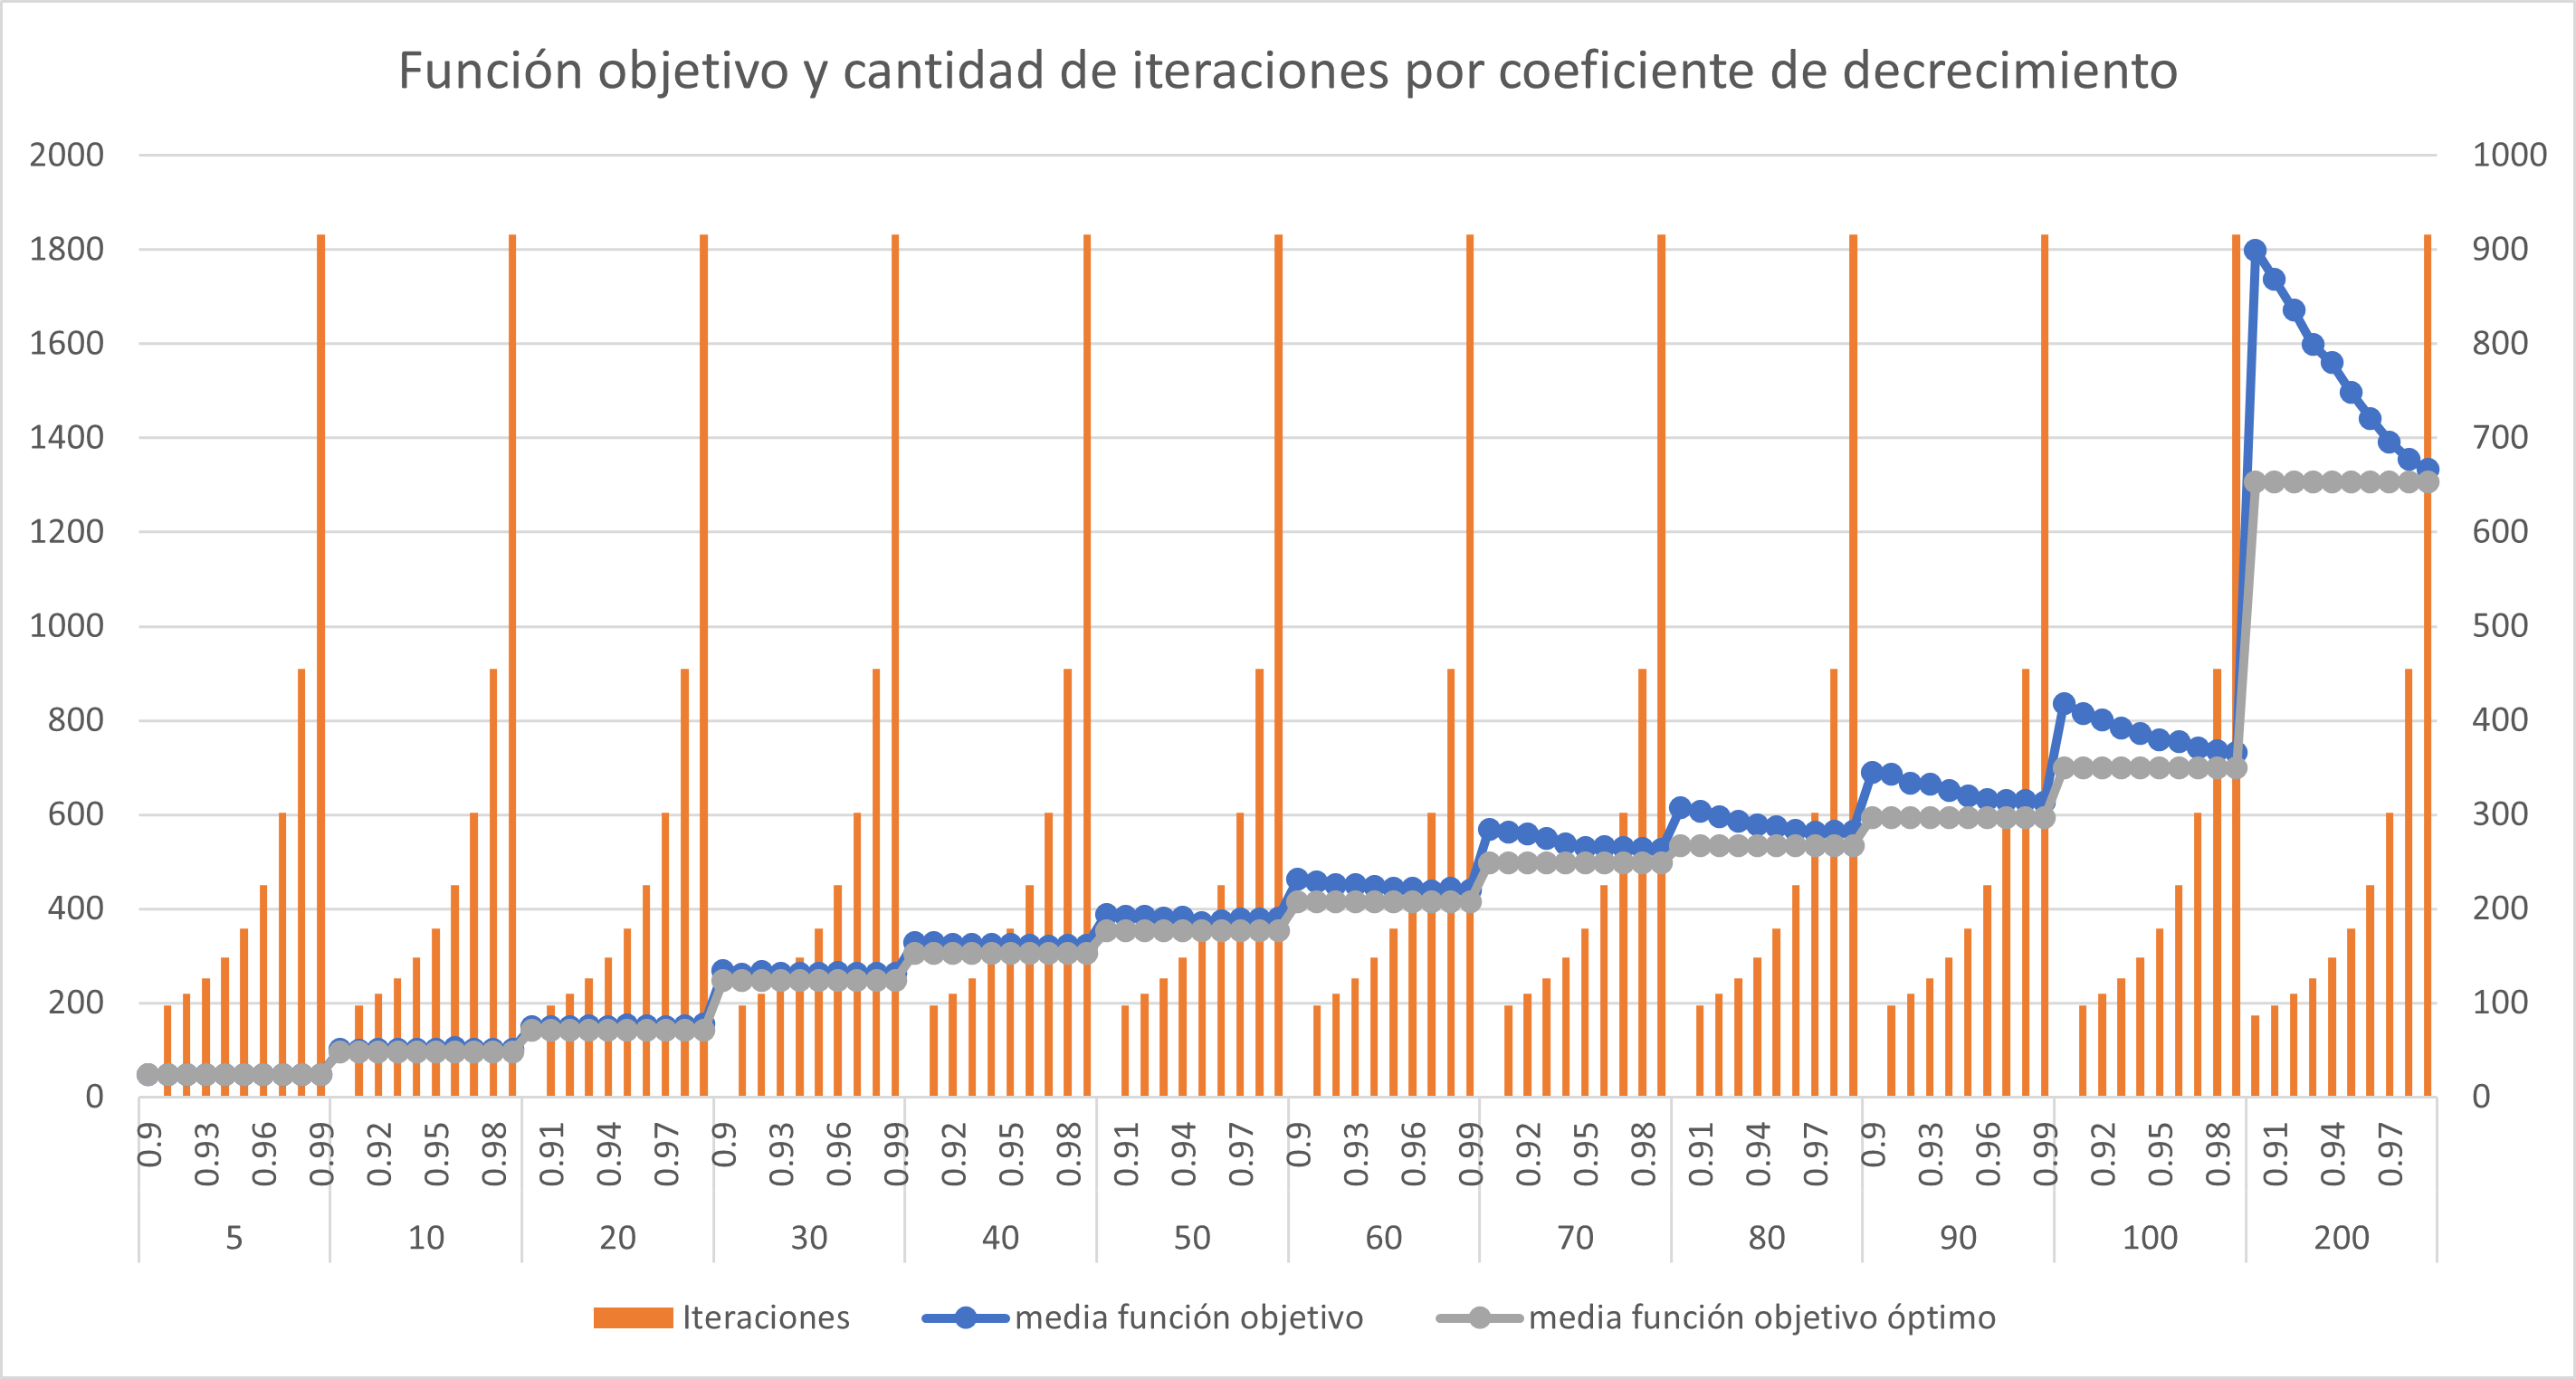
\includegraphics[width=\textwidth]{images/testing/funcion_objetivo_vs_k.png}
    \caption{Función objetivo y cantidad de iteraciones por coeficiente de decrecimiento para todas las instancias.}
    \label{graph:k_all_instances}
\end{figure}

Luego de la experimentación se realizó un gráfico resumen \ref{graph:k_all_instances} que muestra el promedio de los óptimos locales obtenidos para cada instancia con cada coeficiente y para la última instancia de dimensión 200 se puede extraer, como se puede ver en la figura \ref{graph:f_i_por_k_instance_200}, que no existe mayor diferencia entre el coeficiente $0.98$ y $0.99$, con el coeficiente $0.98$ se logra una diferencia entre el óptimo local encontrado por la prueba y el óptimo de referencia de $48.2614$ puntos, con cerca de $455$ iteraciones a diferencia de lo que sucede con el coeficiente $0.99$ que se logra una diferencia de $26.4274$ con casi el doble de iteraciones, siendo casi despreciable en comparación con la diferencia del orden de los $492.4654$ que alcanza el coeficiente $0.90$.

En cambio para una instancia pequeña como la de dimensión 5, ver figura \ref{graph:f_i_por_k_instance_5}, un coeficiente $0.90$ o $0.99$ no afecta en la búsqueda, de hecho siempre se obtiene el óptimo local de referencia, la única gran diferencia es que para un coeficiente de $0.90$, se ejecutan 87 iteraciones y para un coeficiente de $0.99$, se realizan 916 iteraciones.

\begin{figure}[!ht]
    \centering
    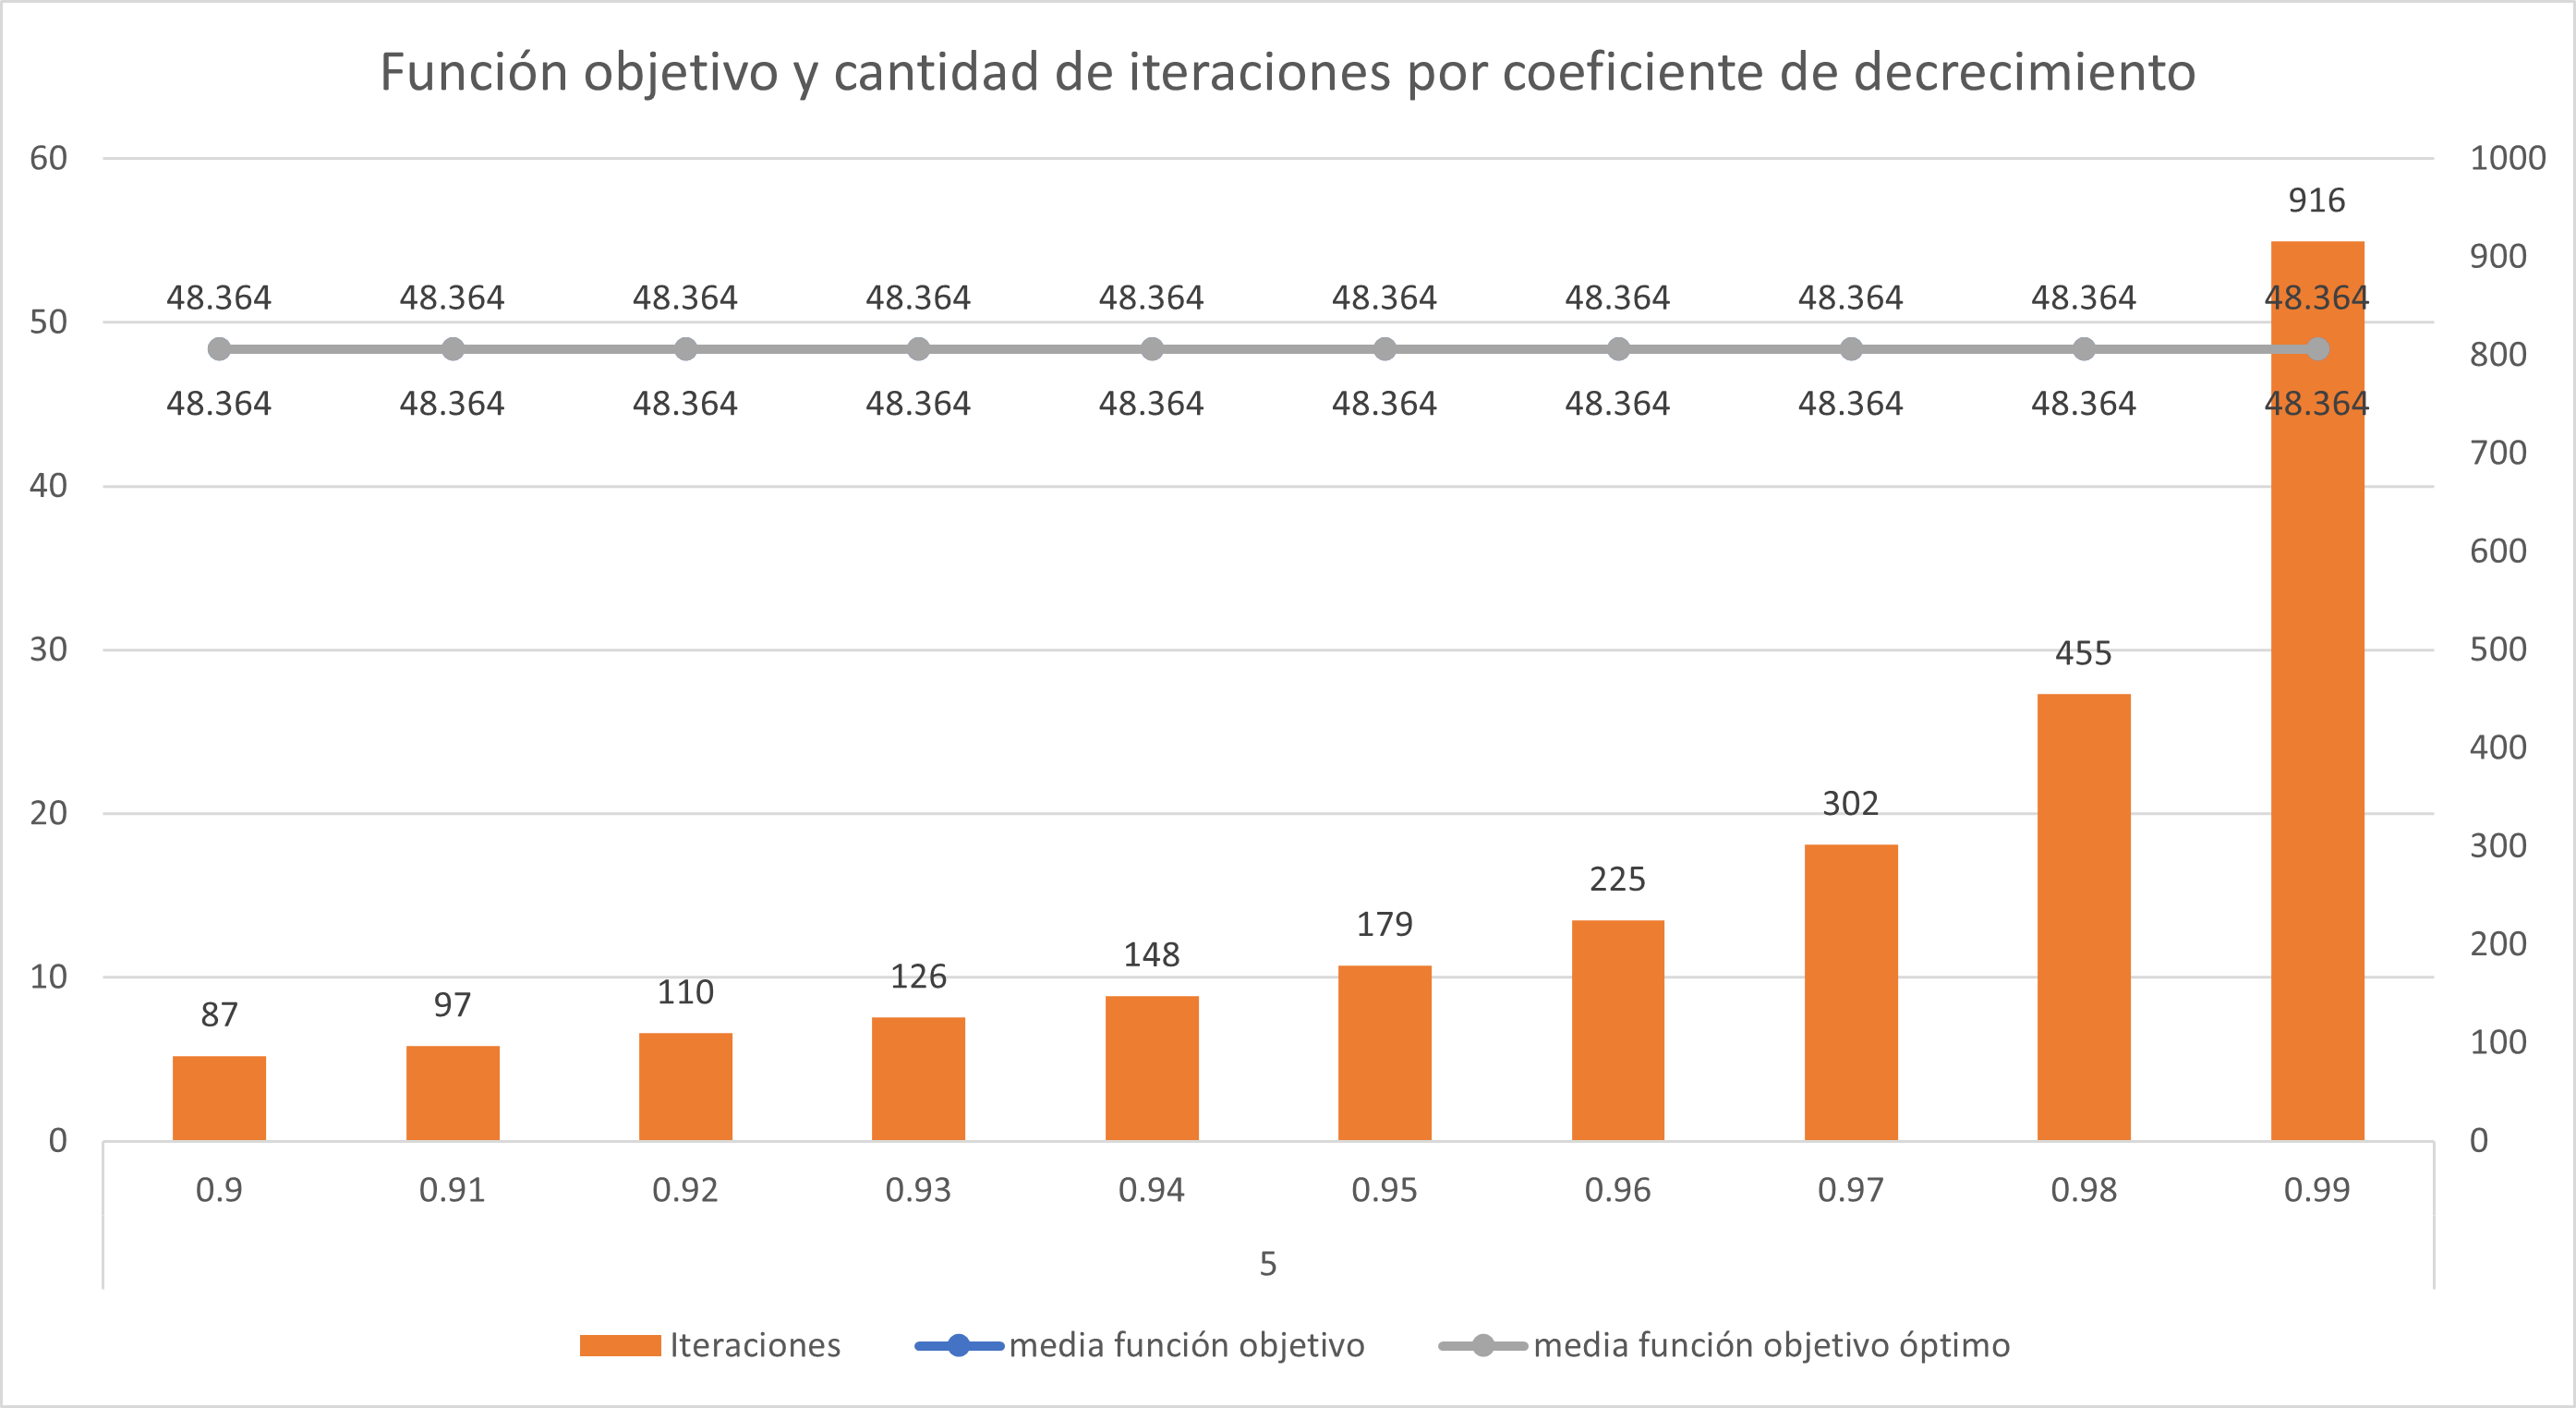
\includegraphics[width=\textwidth]{images/testing/funcion_objetivo_vs_k_5.png}
    \caption{Función objetivo y cantidad de iteraciones por coeficiente de decrecimiento para la instancia de dimensión 5.}
    \label{graph:f_i_por_k_instance_5}
\end{figure}

\begin{figure}[!ht]
    \centering
    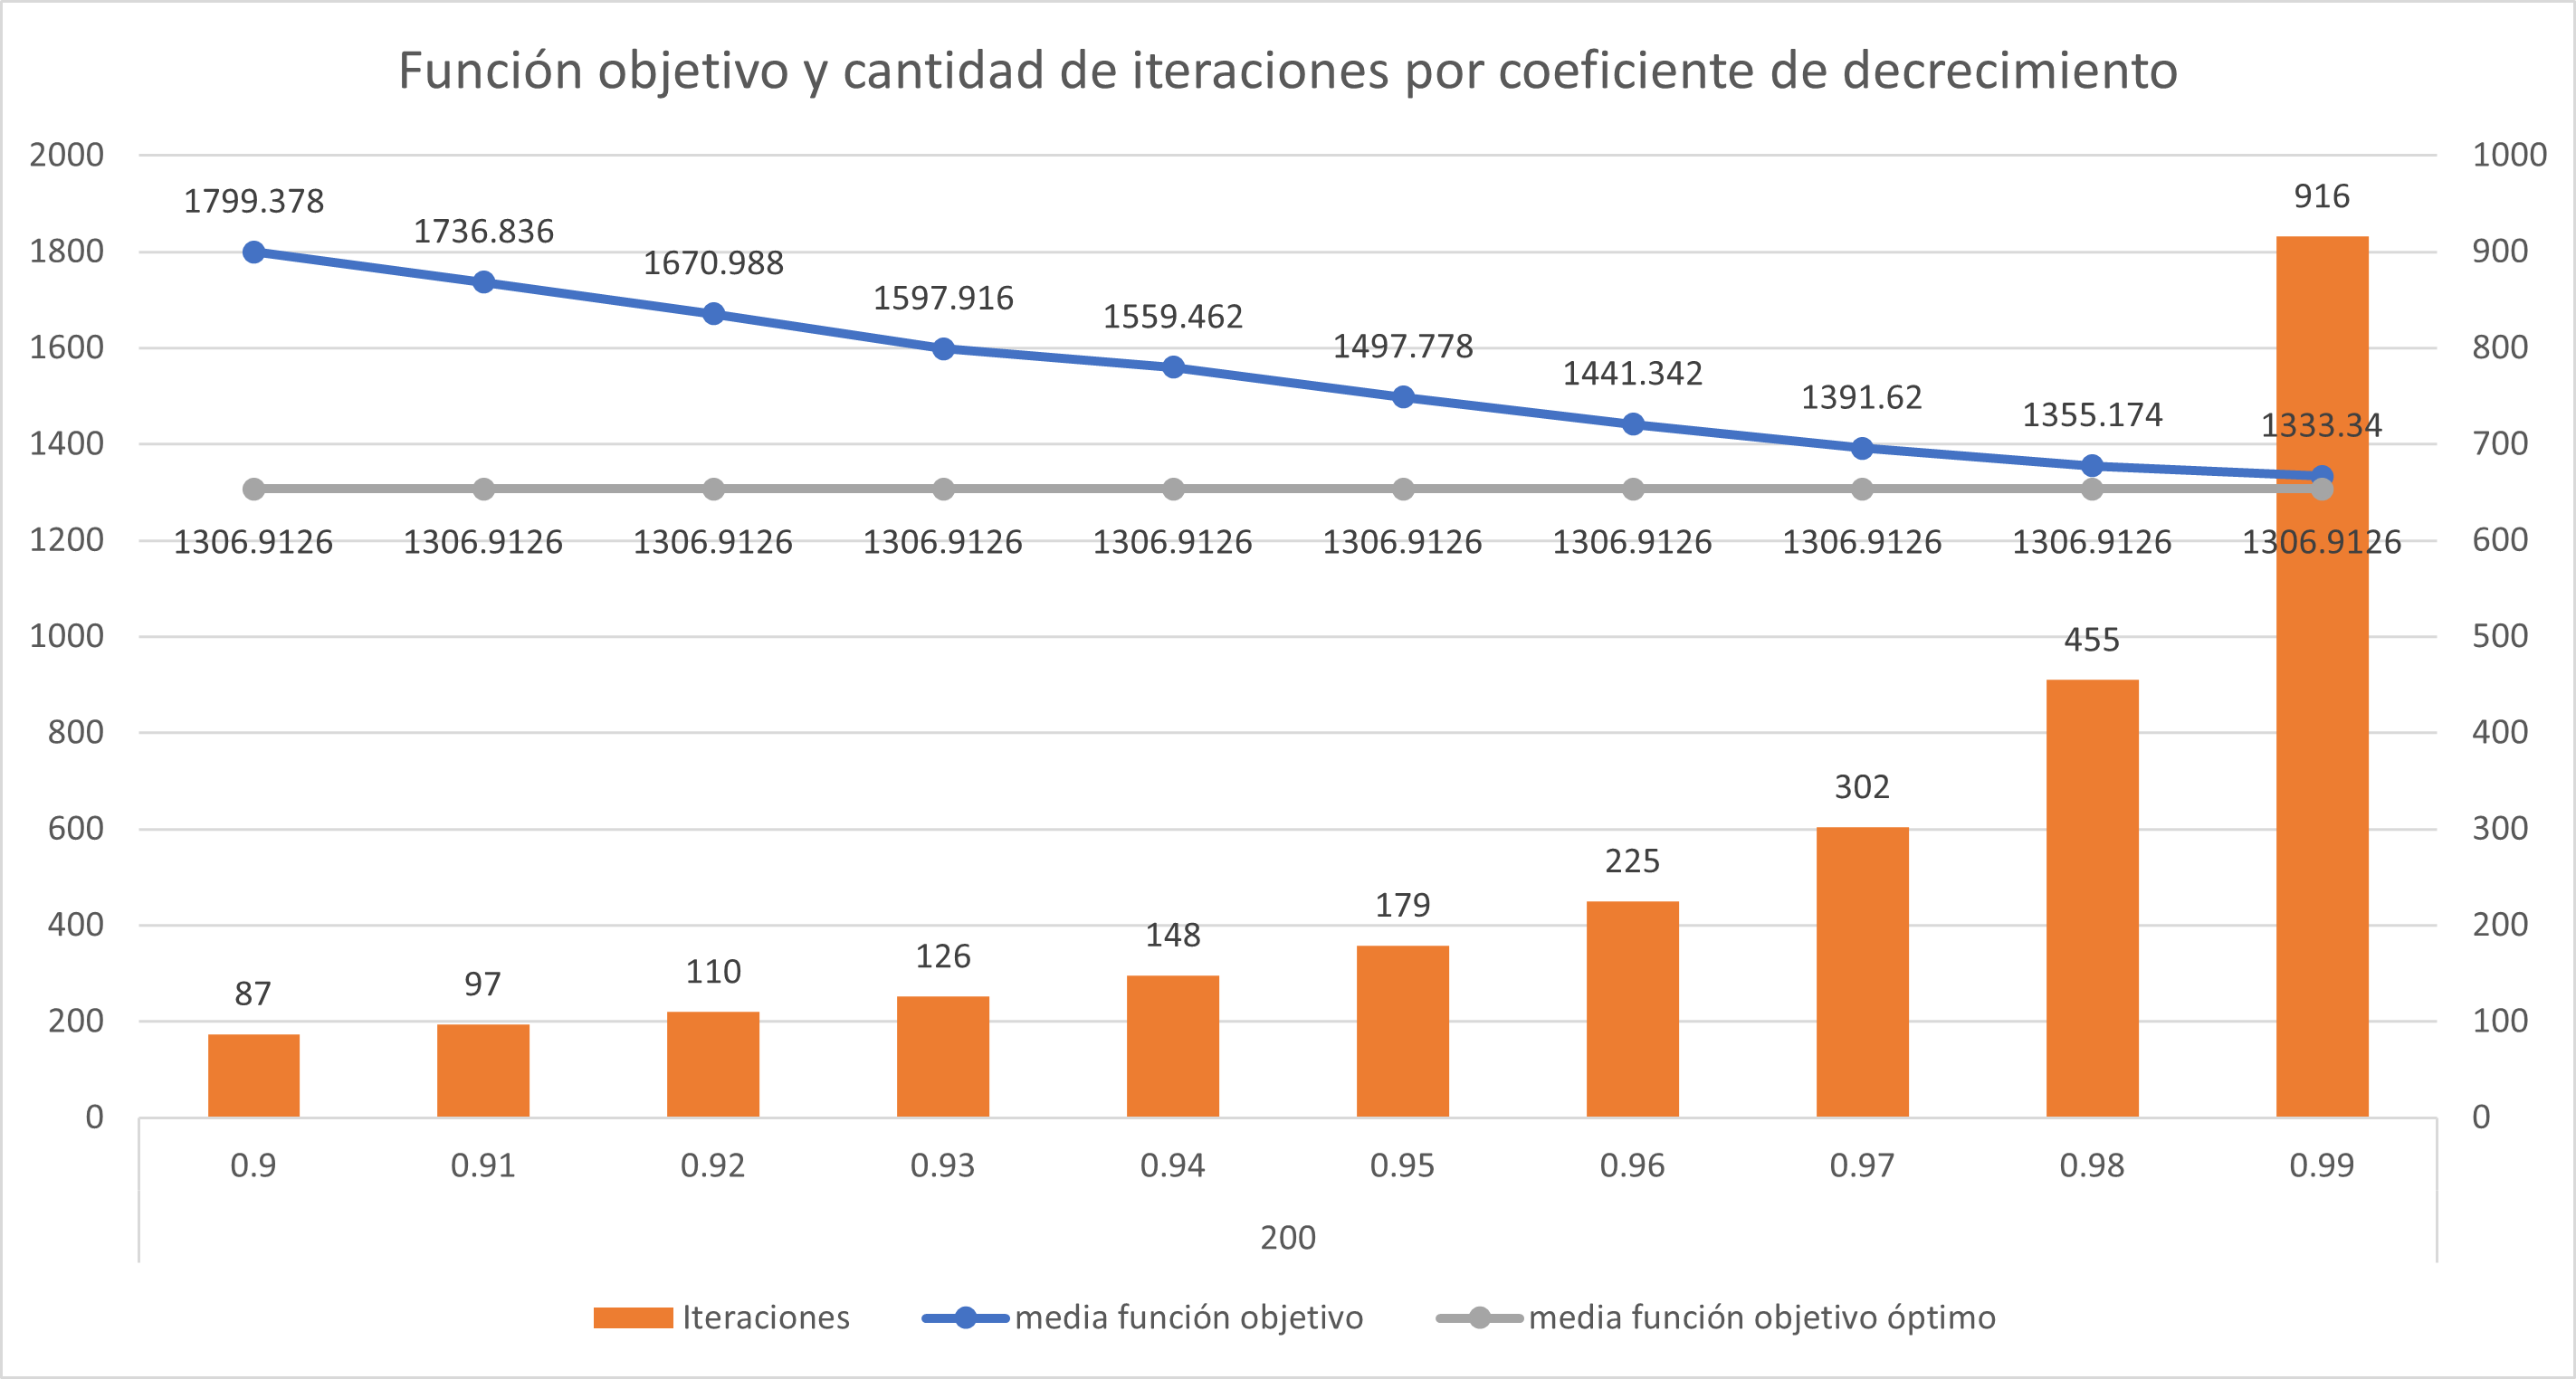
\includegraphics[width=\textwidth]{images/testing/funcion_objetivo_vs_k_200.png}
    \caption{Función objetivo y cantidad de iteraciones por coeficiente de decrecimiento para la instancia de dimensión 200.}
    \label{graph:f_i_por_k_instance_200}
\end{figure}

\subsubsection{Análisis}

Se puede entonces ahora determinar que el coeficiente $0.98$ es un de los mejores coeficientes para encontrar un óptimo aceptable para realizar pruebas, debido a la insignificante diferencia entre los óptimos locales que generan los coeficientes $0.99$ y $0.98$, y la inmensa diferencia entre su cantidad de iteraciones $916$ y $455$, respectivamente

\subsection{Movimiento}

\subsubsection{Logro de la experimentación}

Con la experimentación se logró identificar que el movimiento 2 que corresponde al movimiento completamente iterativo, como se dijo desde un principio no es óptimo para este problema.

Además se identificó una pequeña diferencia entre el movimiento 0 y el 1, como muestran los gráficos \ref{graph:movements_5} y \ref{graph:movements_200}, que representan la media de la función objetivo por movimiento para las instancias $5$ y $200$. Si bien el \textit{movimiento 0} se comporta de mejor manera que el \textit{movimiento 1} en la instancia $200$, no es mucho mejor, solamente una diferencia del orden de los $20$ puntos destructivos. Y se destaca la dificultad que tiene el \textit{movimiento 0} para lograr alcanzar el óptimo de referencia en la instancia de dimensión 5.


\begin{figure}[!ht]
    \centering
    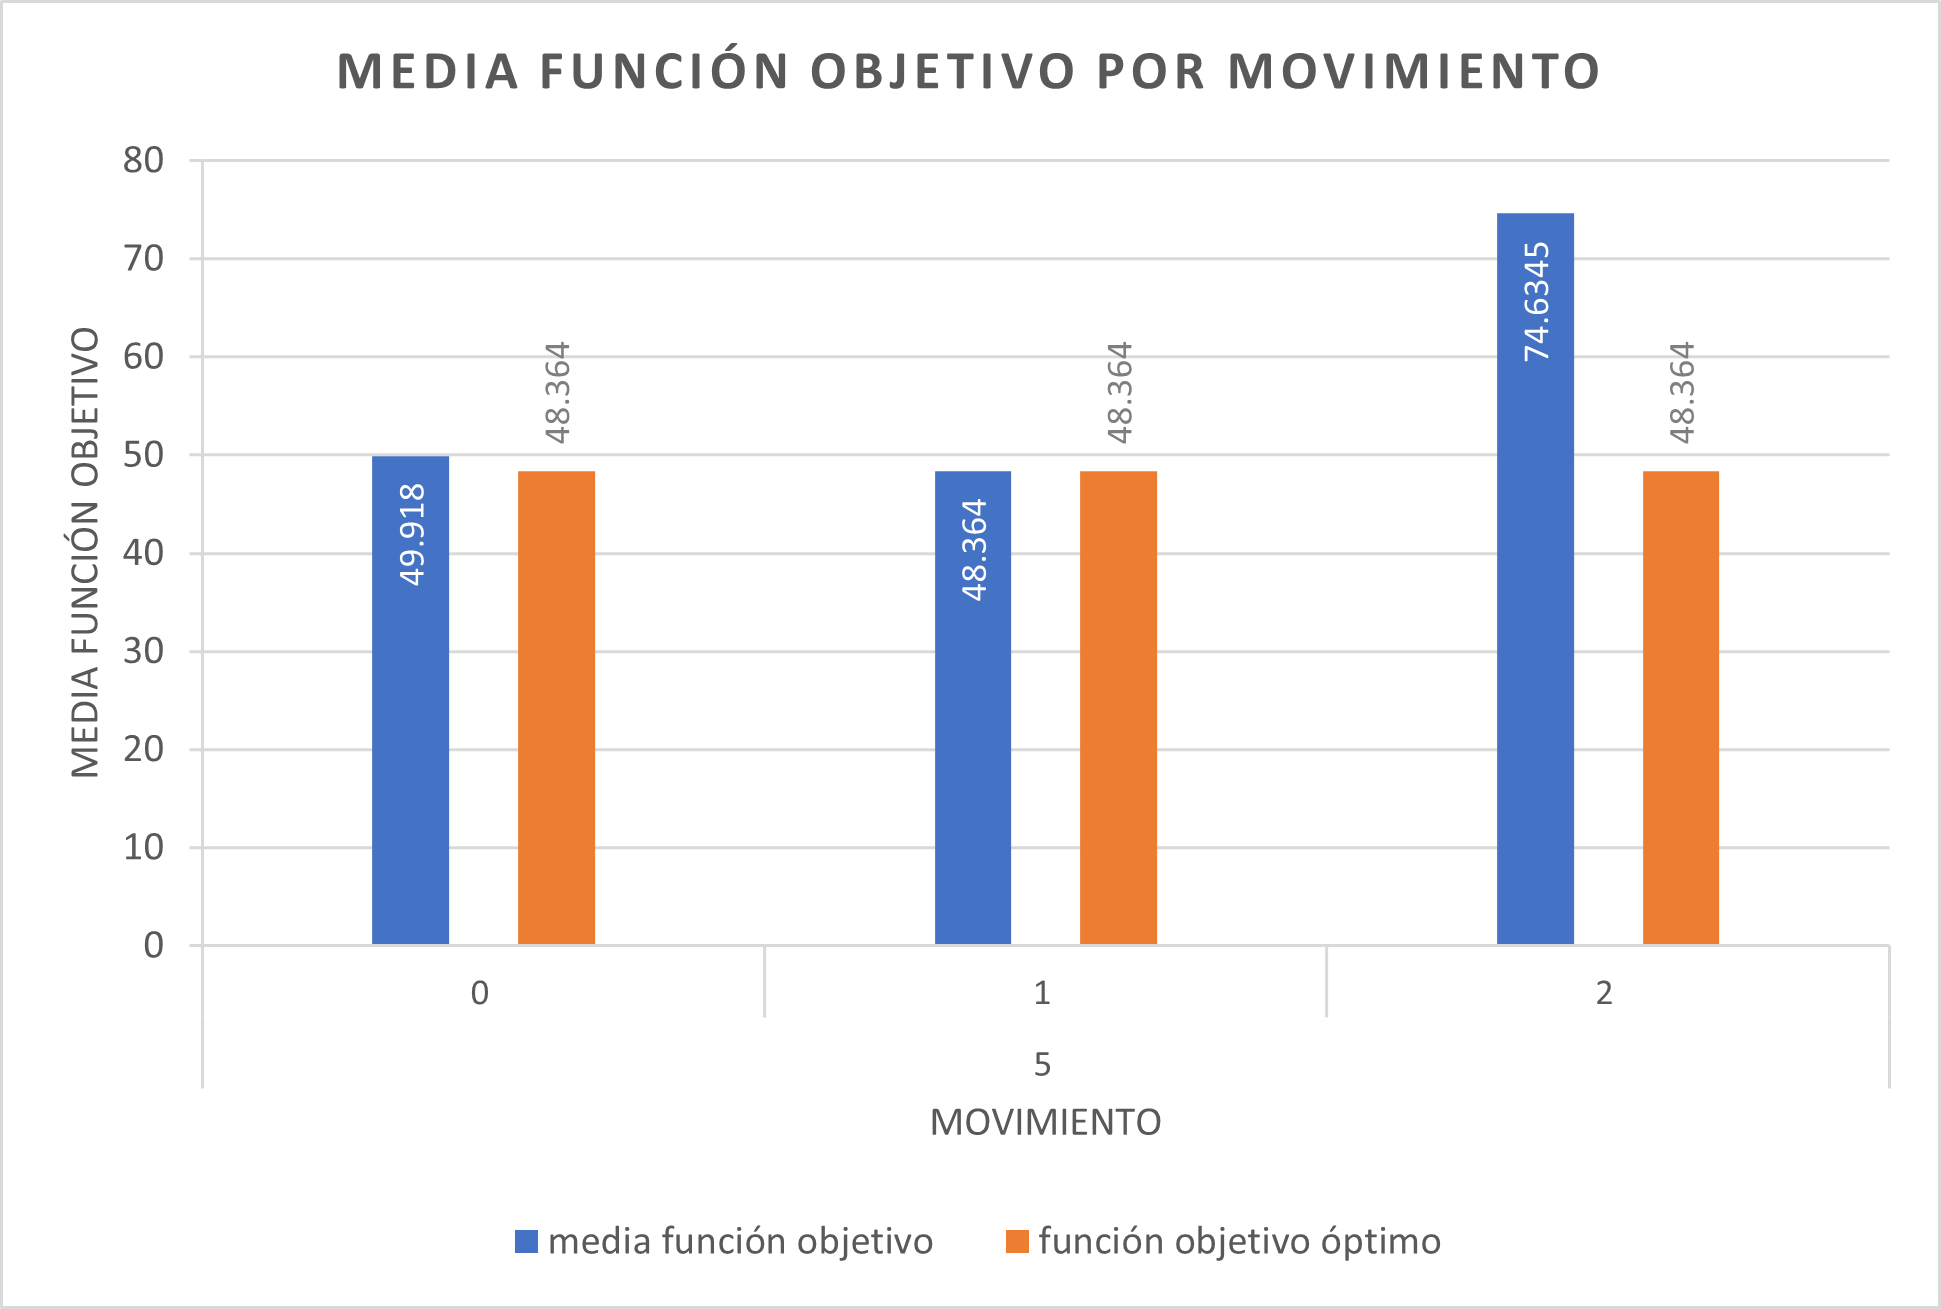
\includegraphics[width=0.8\textwidth]{images/testing/media_por_movimiento_5.png}
    \caption{Media de función objetivo por movimiento para la instancia de dimensión 5.}
    \label{graph:movements_5}
\end{figure}

\begin{figure}[!ht]
    \centering
    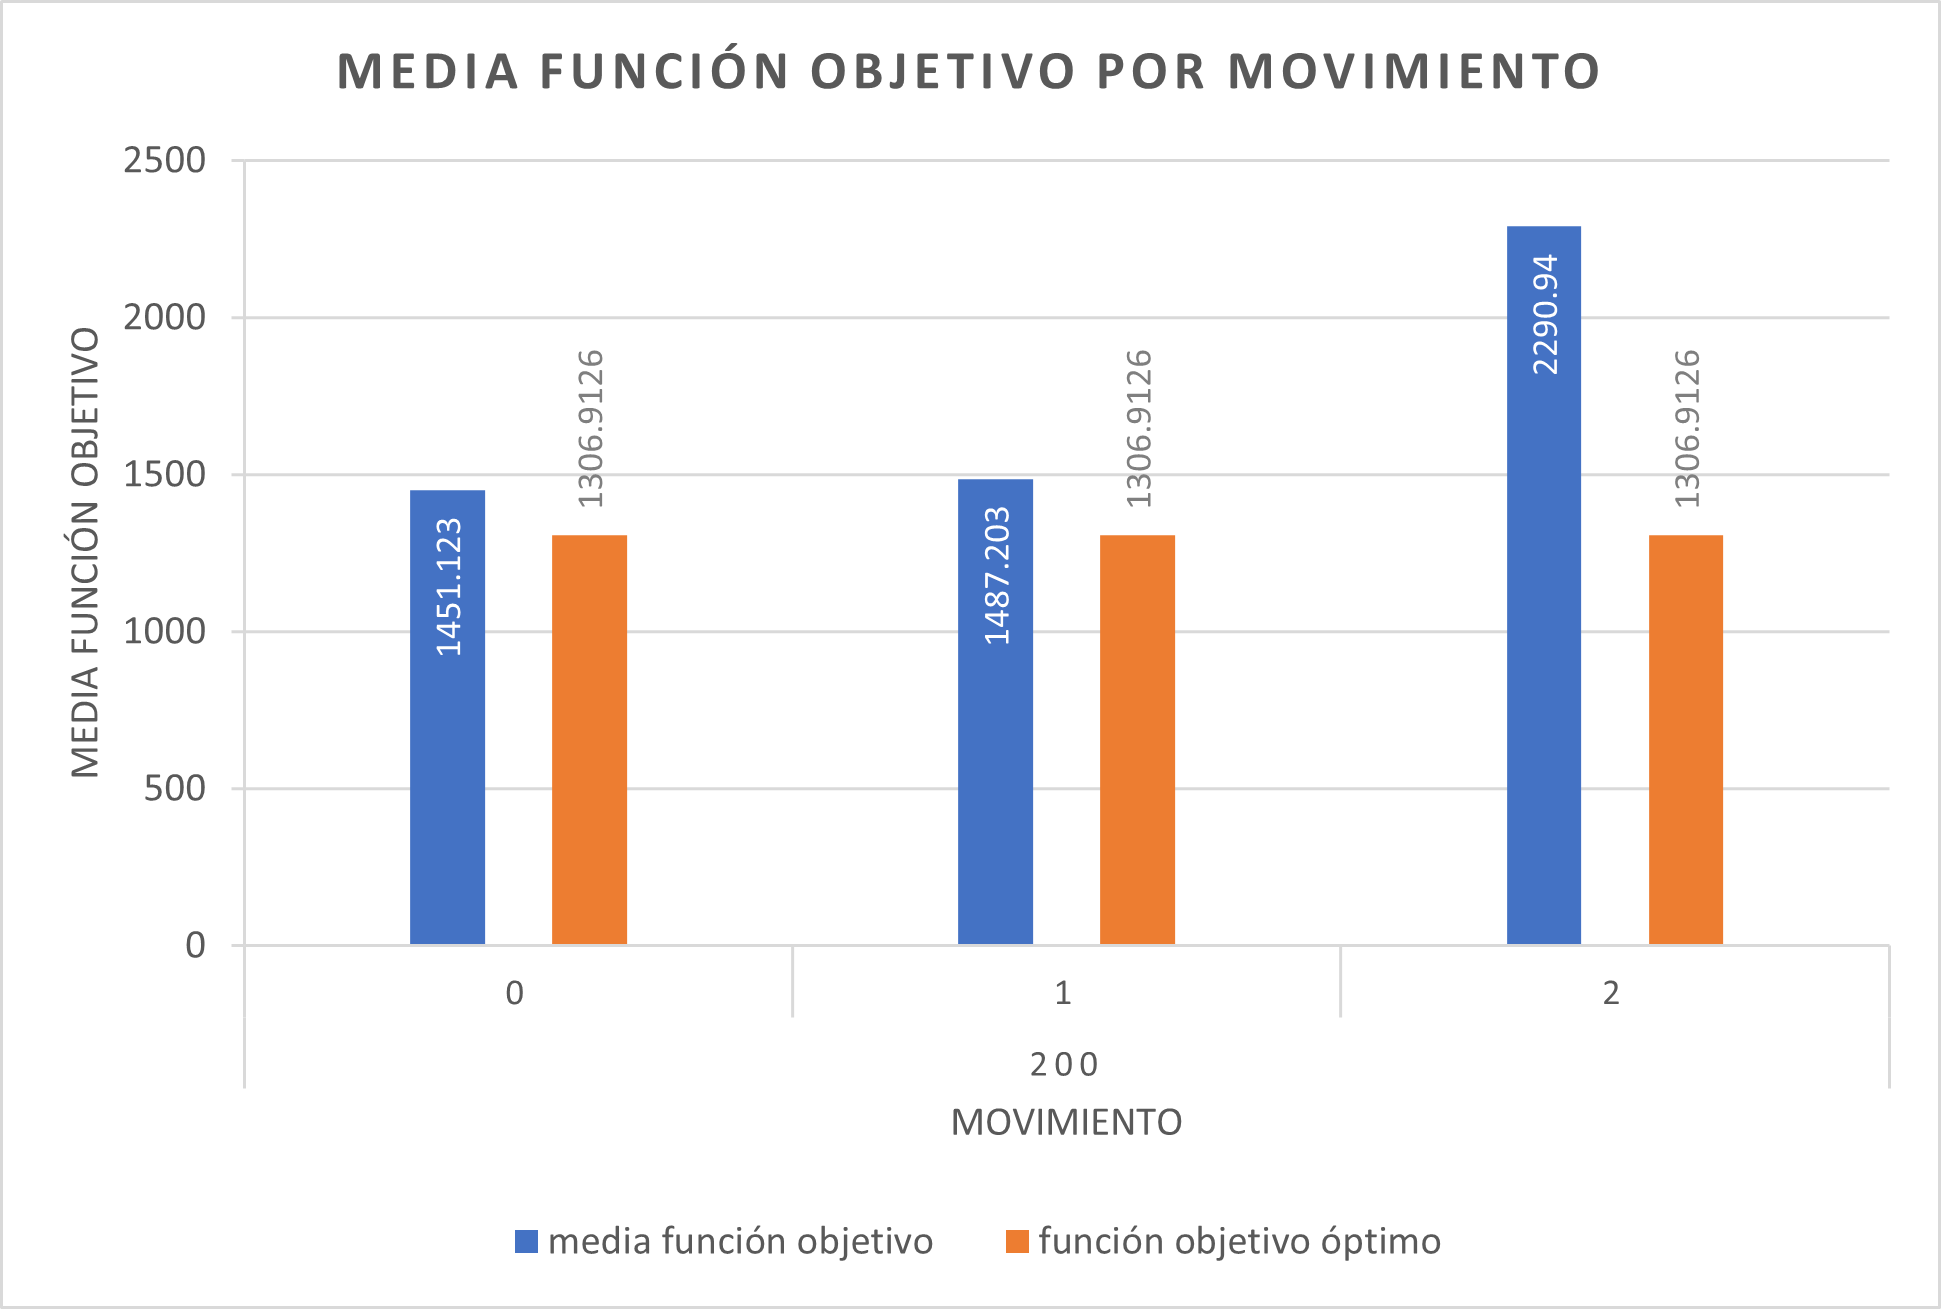
\includegraphics[width=0.8\textwidth]{images/testing/media_por_movimiento_200.png}
    \caption{Media de función objetivo por movimiento para la instancia de dimensión 200.}
    \label{graph:movements_200}
\end{figure}

\subsubsection{Comparación configuraciones}
% - Compare diferencias entre configuraciones distintas de los experimentos.

Para comprar se realizó un gráfico , ver figura \ref{graph:movements}, que muestra los 3 movimientos, de este gráfico se realizó uno similar que muestra solamente los resultados para las instancias $5$ y $200$. 

\begin{figure}[!ht]
    \centering
    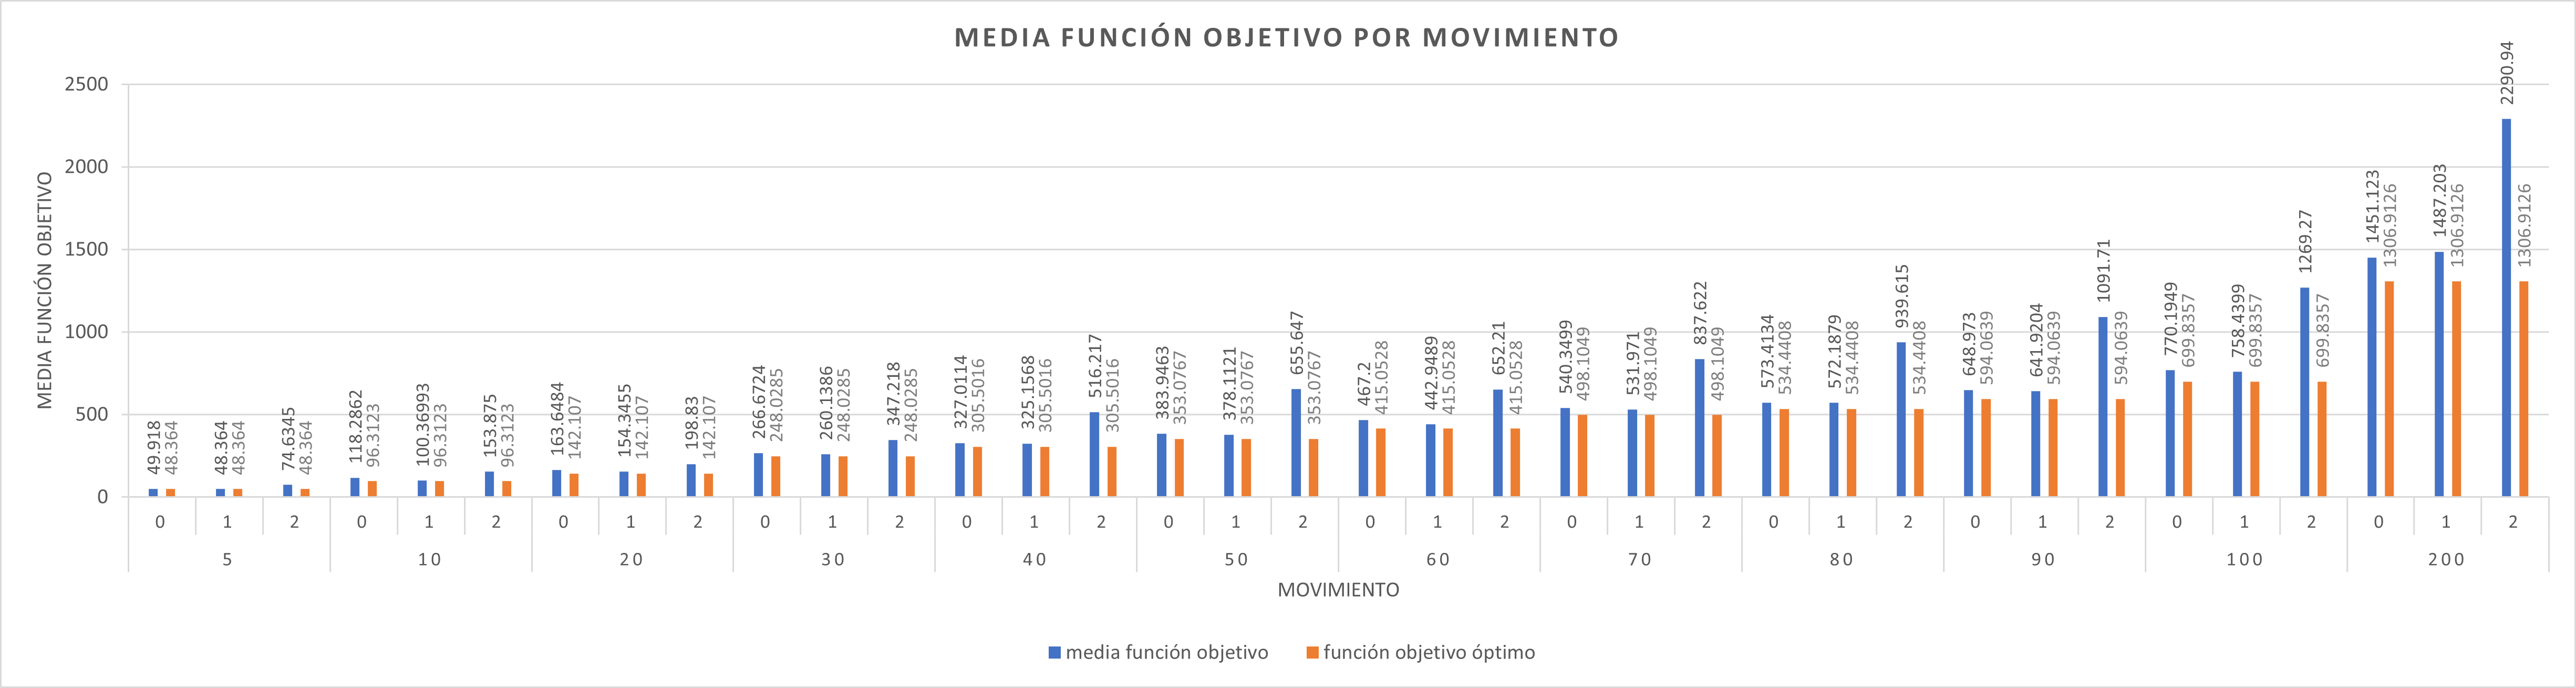
\includegraphics[width=\textwidth]{images/testing/media_por_movimiento.png}
    \caption{Media de función objetivo por movimiento.}
    \label{graph:movements}
\end{figure}

\subsubsection{Análisis}

Para esta experimentación resulta difícil mencionar un movimiento que funcione de la forma más óptima posible para todas las instancias, pero se puede concluir que el movimiento 0 funciona de buena forma para instancias grandes como la 200 pero para instancias pequeñas se aleja un poco del óptimo referencial, el \textit{movimiento 1} funciona de buena manera para las instancias pequeñas y para las más grandes se acerca bastante al óptimo referencial, y el \textit{movimiento 2} no se acerca en absoluto de forma óptima al valor referencial del valor de destrucción.

Un punto destacable es el funcionamiento óptimo para una instancia específica del \textit{movimiento 0}, este movimiento solamente funciona mejor que el \textit{movimiento 1} para la instancia 200, esto puede deberse a algún error en la experimentación o alguna injerencia en la dimensión de la instancia.



\section{Conclusiones}

%  \cite[pág 21]{Introduccion}
%  \cite[pág 21]{Background}
%  \cite[pág 21]{WithTechniques}

% todas las técnicas resuelven el mismo problema o hay algunas diferencias?
% en qué se parecen o difieren las técnicas en el contexto del problema?
% qué limitaciones tienen?
% qué tecnicas o estrategias son las más prometedoras?
% existe trabajo futuro por realizar?
% qué ideas usted propone como lineamientos para continuar con investigaciones futuras?

% Las conclusiones se derivan del trabajo anterior y no hay suficiente desarrollo que avale lo expresado en esta sección.

Luego de realizar las experimentaciones expuestas se logró determinar que para este algoritmo de búsqueda local que combina la técnica \textit{Simulated Annealing} con \textit{Mejor mejora}, existe dependencia entre el coeficiente de decrecimiento y la cantidad de iteraciones de la búsqueda, además se logró determinar la injerencia de la precisión del coeficiente de decrecimiento, habiendo acordado el coeficiente $0.98$ como el más óptimo para realizar pruebas o ejecuciones de escenarios de dimensión alta para el entorno de experimentación presentado en el informe.

Además se logró determinar que los movimiento 0 y 1, que presentan cierto grado de aleatoriedad, funcionan de forma óptima para las instancias propuestas por la literatura de referencia \cite{sonuc-2017}.
Por último se destaca la imposibilidad de lograr llegar al óptimo local de referencia, no se pudo determinar si este problema es por la modificación que se hizo al algoritmo, agregándole la heurística \textit{Mejor Mejora} o algún error en la implementación tanto del algoritmo como la calibración de los parámetros.

Queda propuesto experimentar con instancias de dimensión mayor a 200 para lograr determinar si el \textit{movimiento 0}, totalmente aleatorio, es realmente un buen movimiento para instancias de dimensiones mayores a las expuestas.


% \section{Bibliograf\'ia}
% Indicando toda la informaci\'on necesaria de acuerdo al tipo de documento revisado. Todas las referencias deben ser citadas en el documento.
\bibliographystyle{plain}
\bibliography{Referencias}

\end{document} 